\section{ \texttt{ex010.PVT.xlsm} - Расчет базовых PVT свойств флюидов}

Расчет физико химических свойств пластовых флюидов (PVT параметров) лежит в основе всех расчетов систем нефтедобычи. При решении прикладных задач редко возникает необходимость расчета PVT свойств непосредственно, однако понимание принципа их расчета, а особенно зависимости результатов расчета от исходных данных важно.
   
Для выполнения упражнения используйте файл \texttt{ex010.PVT.xlsm} (смотри рис. \ref{ris:Ex10_1}).

\begin{figure}[h!]
	\center{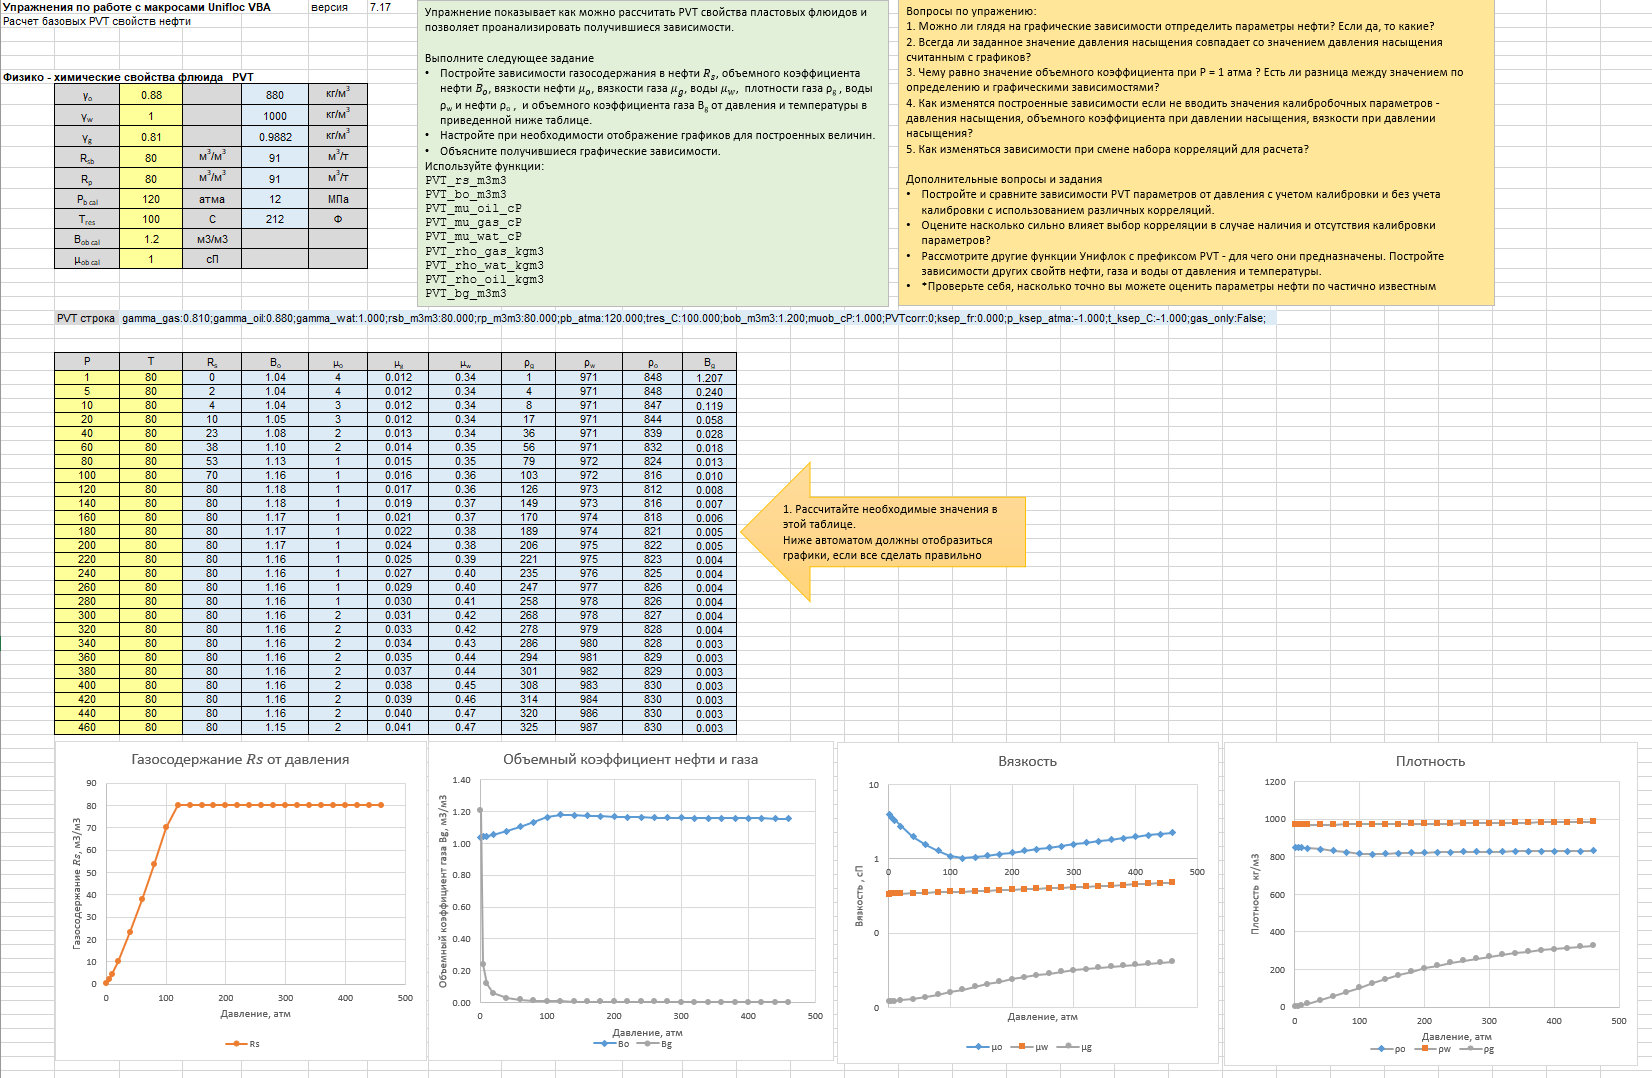
\includegraphics[width=1\linewidth]{Ex10_1}}
	\caption{Упражнение \texttt{ex010.PVT.xlsx} со всеми заполненными полями.}
	\label{ris:Ex10_1}
\end{figure}

\subsection{Упражнение}
Упражнение показывает как рассчитать PVT свойства пластовых флюидов и позволяет проанализировать получившиеся зависимости. 

Выполните следующие задания
\begin{enumerate}
	\item  Постройте зависимости газосодержания в нефти $R_s(P,T)$, объемного коэффициента нефти $B_o(P,T)$, вязкости нефти $\mu_o(P,T)$, вязкости газа $\mu_g(P,T)$, воды $\mu_w(P,T)$,  плотности газа $\rho_g(P,T)$ , воды $\rho_w(P,T)$ и нефти $\rho_o(P,T)$ ,  и других PVT параметров от давления и температуры. 
	
	\item  Убедитесь, что для всех построенных графиков вы понимаете их поведение при изменении давления и температуры. 
	
\end{enumerate}

Для выполнения расчетов используйте функции \unf{} начинающиеся с префикса \texttt{PVT\_}:




\subsection{Вопросы для самоконтроля}
Для самоконтроля ответьте на следующие вопросы:

\begin{enumerate}
	
	\item Можно ли глядя на графические зависимости определить параметры нефти? Если да, то какие?
	
	\item Всегда ли заданное значение давления насыщения совпадает со значением считанным с графиков?
	
	\item Чему равно значение объемного коэффициента $B_o$ при $P = 1$ атма? Есть ли разница между значением по определению и графическими зависимостями? Если разница есть, то каким параметром она может быть вызвана? Постройте график иллюстрирующий данную зависимость.
	
	\item Чему равно значение газосодержания $r_s$ при $P = 1$ атма? Есть ли разница между значением по определению и графическими зависимостями? Если разница есть, то каким параметром она может быть вызвана? Постройте график иллюстрирующий данную зависимость.
	
 	\item Как изменятся построенные зависимости если не вводить значения калибровочных параметров - давления насыщения, объемного коэффициента при давлении насыщения, вязкости при давлении насыщения?
	
	\item 	Как изменяться зависимости PVT параметров от давления и температуры при смене набора корреляций для расчета?
	
\end{enumerate}

\subsection{Дополнительные вопросы и задания}

	Для того, чтобы глубже разобраться в расчете свойств флюидов с использованием \unf{} ответьте на дополнительные вопросы, которые легко превращаются в задания.

\begin{enumerate}
	
	\item Постройте и сравните зависимости PVT параметров от давления с учетом калибровки и без учета калибровки с использованием различных корреляций. Что важнее - правильно выбрать корреляцию или задать корректные калибровочные параметры?
	
	\item Оцените насколько сильно влияет выбор корреляции в случае наличия и отсутствия калибровки параметров?
	
	\item Рассмотрите другие функции Унифлок с префиксом PVT - для чего они предназначены. Постройте зависимости других свойтв нефти, газа и воды от давления и температуры. 
	
	\item *Проверьте себя, насколько точно вы можете оценить параметры нефти по частично известным данным? Какой минимальный набор данных надо знать? Проверьте коллег попросив их оценить/угадать свойства нефти по частичным данным. 
	
	\item Простой пример - часто нет данных по плотности газа (например в технологическом режиме добывающих скважин). Можно ли восстановить этот параметр по другим данным?
	
	\item Можно ли оценить величину газосодержания нефти по плотности нефти и газа?
	
	\item Можно ли оценить плотность нефти по газосодержанию и давлению насыщения?
	
\end{enumerate}


\section{\texttt{ex011.MF\_gas\_fraction.xlsm} - Расчет свойств потока флюидов}

PVT функции описывают свойства флюидов. Можно представить себе, что они описывают свойства флюидов находящихся в PVT бомбе - устройстве для отбора проб. В этом случае флюиды неподвижны и находятся в равновесном состоянии. На практике приходится иметь дело с флюидами двигающимися в скважине или трубопроводе - с потоком флюидов. В потоке флюидов добавляются дополнительные параметры -- расход флюидов или дебит $Q_{liq}, Q_g$ и обводненность $f_w$ -- показатель показывающий объемную долю воды в потоке. 
Функции работающие с потоками в \unf{} имеют префикс \mintinline{vb.net}{MF_}. Префикс должен намекать на многофазность потока и на самом деле плох с лингвистической точки зрения (multiphase - has no F letter), но удобен с программистской точки зрения и уже поздно его менять.

Файл примера \texttt{ex011.MF\_gas\_fraction.xlsm} можно найти в папке \texttt{exercises} репозитория \unf{} (смотри рис. \ref{ris:Ex11_1}).

\begin{figure}[h!]
	\center{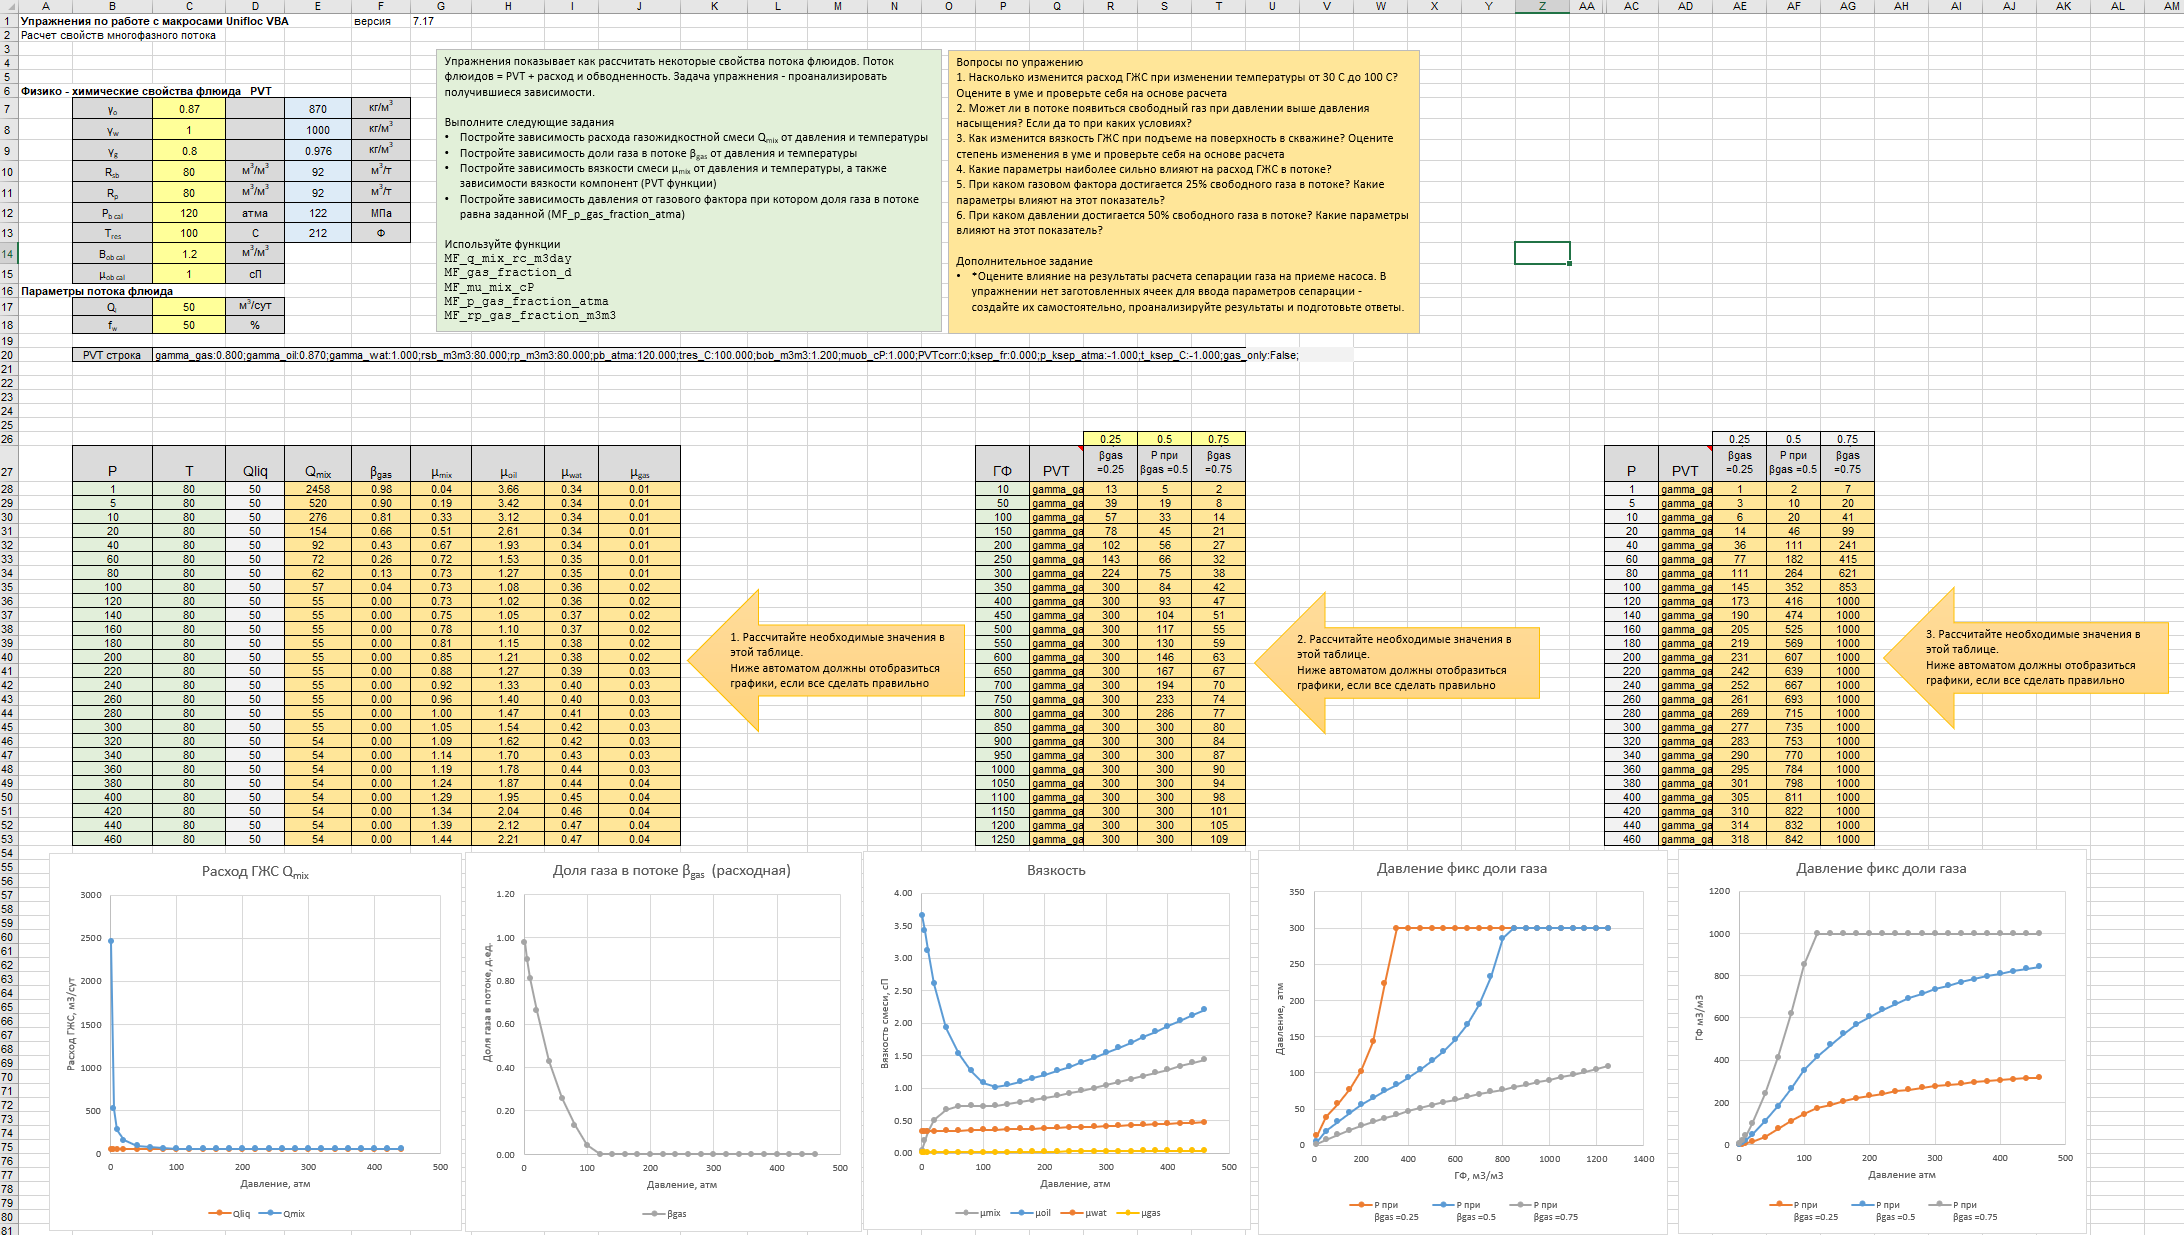
\includegraphics[width=1\linewidth]{Ex11_1}}
	\caption{Упражнение \texttt{ex011.MF\_gas\_fraction.xlsm}  со всеми заполненными полями }
	\label{ris:Ex11_1}
\end{figure}

\subsection{Упражнение}
Упражнение показывает как рассчитать некоторые свойства потока флюидов. Поток флюидов = PVT + расход и обводненность. Задача упражнения - проанализировать получившиеся зависимости.

Выполните следующие задания
\begin{enumerate}
	\item Постройте зависимость расхода газожидкостной смеси $Q_{mix}(P,T)$ от давления $P$ и температуры $T$; 
	\item Постройте зависимость доли газа в потоке $\beta_{gas}(P,T)$ от давления $P$ и температуры $T$;
	\item Постройте зависимость вязкости смеси $\mu_{mix}(P,T)$ от давления $P$ и температуры $T$, а также зависимости вязкости отдельных компонент от давления $P$ и температуры $T$; 
	\item Постройте зависимость давления  от газового фактора $P(R_p)$ при котором доля газа в потоке  равна заданной  $P(R_p)|_{\beta_{gas} = const}$;
	
	\item Постройте зависимость газового фактора от давления $R_p(P)$  при котором доля газа в потоке равна заданной $R_p(P)|_{\beta_{gas} = const}$; 
 	
\end{enumerate}

Для выполнения расчетов используйте следующие функции \unf{}:
\begin{itemize}

	\item \texttt{MF\_q\_mix\_rc\_m3day}
	\item \texttt{MF\_gas\_fraction\_d}
	\item \texttt{MF\_mu\_mix\_cP}
	\item \texttt{MF\_p\_gas\_fraction\_atma}
	\item \texttt{MF\_rp\_gas\_fraction\_m3m3}

\end{itemize}

Убедитесь, что для всех построенных графиков вы понимаете их поведение при изменении давления и температуры. 

\subsection{Вопросы для самоконтроля}
Для самоконтроля ответьте на следующие вопросы:

\begin{enumerate}
	
	\item Насколько изменится расход ГЖС при изменении температуры от 30 \textdegree С до 100 \textdegree С? Оцените ответ в уме и проверьте себя на основе расчета. Что еще надо учесть кроме температуры?
	
	\item Может ли в потоке появиться свободный газ при давлении выше давления насыщения? Если да то при каких условиях?
	
	\item Как изменится вязкость ГЖС при подъеме на поверхность в скважине? Оцените степень изменения в уме и проверьте себя на основе расчета.
	
	\item Какие параметры наиболее сильно влияют на расход ГЖС в потоке?
	
	\item При каком газовом факторе достигается 25\% свободного газа в потоке? Какие параметры влияют на этот показатель?
	 	
	\item При каком давлении достигается 50\% свободного газа в потоке? Какие параметры влияют на этот показатель?
	 	
\end{enumerate}

\subsection{Дополнительные вопросы и задания}

Для того, чтобы глубже разобраться в расчете свойств флюидов с использованием \unf{} ответьте на дополнительные вопросы, которые легко превращаются в задания.

\begin{enumerate}
	
	\item *Оцените влияние на результаты расчета сепарации газа на приеме насоса. В упражнении нет заготовленных ячеек для ввода параметров сепарации - создайте их самостоятельно, проанализируйте результаты и подготовьте ответы.
	
	
	
\end{enumerate}


В дополнительном задании говорится о сепарации газа на приеме насоса. Имеется в виду следующее - если у нас есть пластовые флюиды, свойства которых мы знаем и можем задать, то после сепарации части свободного газа, что часто происходит на скважинном насосе, свойства флюида изменятся. Изменится его эффективное давление насыщения (потому что мы убрали часть газа) и газосодержание при давлении насыщения. И соответственно поплывут и остальные свойства. Это можно учесть задав в \mintinline{vb.net}{PVT_Encode()} три параметра - коэффициент сепарации газа $K_{sep}$, давление при которой произошла сепарации $P_{sep}$ и температуру при которой произошла сепарация $T_{sep}$. Подробнее про это можно найти в соответствующих разделах (поэтому тут это задание дополнительное).

\section{\texttt{ex012.PVT\_z\_factor.xlsm} - Пример расчета свойств газа}

Как рассчитать коэффициент сверхсжимаемости газа и какие могут быть неожиданности. 

\section{\texttt{ex013.PVT\_hydrates.xlsm} - Расчет кривой образования гидратов}

Пример показывает, как можно оценить кривые образования гидратов
